\documentclass[aspectratio=169,10pt,t]{beamer}

\usepackage[T1]{fontenc}
\usepackage[utf8]{inputenc}
\usepackage{lmodern}
\usepackage{microtype}
\usepackage{amsmath,amssymb}
\usepackage{booktabs}
\usepackage{array}
\usepackage{tabularx}
\usepackage{colortbl}
\usepackage{graphicx}
\usepackage{tikz}
\usetikzlibrary{arrows.meta,positioning,shapes.geometric,calc,fit,backgrounds}
\usepackage{pgfplots}
\pgfplotsset{compat=1.18}
\usepackage{listings}
\usepackage{qrcode}
\usepackage{hyperref}

\graphicspath{{figures/}}

\definecolor{rPrimary}{RGB}{27,38,79}
\definecolor{rSecondary}{RGB}{42,72,145}
\definecolor{rAccent}{RGB}{233,151,42}
\definecolor{rTeal}{RGB}{0,150,136}
\definecolor{rBg}{RGB}{245,247,251}
\definecolor{rInk}{RGB}{32,36,45}
\definecolor{rMuted}{RGB}{108,116,132}
\definecolor{rRed}{RGB}{190,55,65}
\definecolor{rLine}{RGB}{205,210,218}
\colorlet{cPNP}{rPrimary}
\colorlet{cCNP}{rAccent}
\colorlet{cCNC}{rTeal}
\colorlet{cCLP}{rSecondary}
\colorlet{cCLC}{rRed}

%% ---------- Theme ----------
\usetheme{default}
\usefonttheme{professionalfonts}
\setbeamertemplate{navigation symbols}{}
\setbeamercolor{normal text}{fg=rInk,bg=white}
\setbeamercolor{structure}{fg=rPrimary}
\setbeamercolor{alerted text}{fg=rAccent}
\setbeamerfont{frametitle}{series=\bfseries,size=\Large}
\setbeamercolor{frametitle}{fg=rPrimary,bg=white}
\setbeamertemplate{itemize item}{\color{rAccent}\scriptsize$\blacktriangleright$}
\setbeamertemplate{itemize subitem}{\color{rSecondary}\scriptsize$\bullet$}
\setbeamertemplate{blocks}[rounded][shadow=false]
\setbeamercolor{block title}{bg=rPrimary,fg=white}
\setbeamercolor{block body}{bg=rBg,fg=rInk}
\setbeamercolor{block title alerted}{bg=rAccent,fg=white}
\setbeamercolor{block body alerted}{bg=rAccent!12,fg=rInk}
\setbeamercolor{block title example}{bg=rTeal,fg=white}
\setbeamercolor{block body example}{bg=rTeal!10,fg=rInk}
\setbeamersize{text margin left=0.58cm,text margin right=0.58cm}

\setbeamertemplate{frametitle}{%
	\nointerlineskip%
	\vspace{0.5em}\hspace{0.7em}%
	\begin{minipage}{\dimexpr0.94\paperwidth-0.7em\relax}%
		{\usebeamerfont{frametitle}\usebeamercolor[fg]{frametitle}\insertframetitle}\par%
	\end{minipage}\par%
	\begin{tikzpicture}[remember picture,overlay]
		\draw[rAccent,line width=2pt]
			([xshift=0.58cm,yshift=-11mm]current page.north west) -- ++(1.45cm,0);
	\end{tikzpicture}%
	\vspace{0pt}%
}

\setbeamercolor{footcol}{fg=white,bg=rPrimary}
\setbeamertemplate{footline}{%
	\leavevmode%
	\hbox{%
		\begin{beamercolorbox}[wd=0.30\paperwidth,ht=2.6ex,dp=1.2ex,leftskip=0.8em]{footcol}%
			\scriptsize Routly
		\end{beamercolorbox}%
		\begin{beamercolorbox}[wd=0.50\paperwidth,ht=2.6ex,dp=1.2ex,center]{footcol}%
			\scriptsize\insertshorttitle
		\end{beamercolorbox}%
		\begin{beamercolorbox}[wd=0.20\paperwidth,ht=2.6ex,dp=1.2ex,rightskip=0.8em]{footcol}%
			\scriptsize\hfill\insertframenumber\,/\,\inserttotalframenumber
		\end{beamercolorbox}%
	}\vskip0pt%
}

\setbeamertemplate{caption}{\raggedright\insertcaption\par}
\setbeamerfont{caption}{size=\scriptsize}
\setbeamercolor{caption name}{fg=rSecondary}

\lstset{
	basicstyle=\ttfamily\tiny,
	columns=fullflexible,
	keepspaces=true,
	showstringspaces=false,
	breaklines=true,
	frame=none,
	aboveskip=1pt,
	belowskip=1pt
}

%% ---------- Helpers ----------
\newcommand{\sectionframe}[3]{%
	\begin{frame}[plain]
		\begin{tikzpicture}[remember picture,overlay]
			\fill[rPrimary](current page.south west) rectangle (current page.north east);
			\fill[rAccent]([yshift=-3mm]current page.west) rectangle ([yshift=0mm]current page.east);
			\node[anchor=west,text=rAccent,font=\Large\bfseries]
			at ([xshift=13mm,yshift=24mm]current page.west) {#1};
			\node[anchor=west,text=white,font=\huge\bfseries,text width=0.82\paperwidth]
			at ([xshift=13mm,yshift=7mm]current page.west) {#2};
			\node[anchor=west,text=rBg,font=\small,text width=0.86\paperwidth]
			at ([xshift=13mm,yshift=-25mm]current page.west) {#3};
		\end{tikzpicture}
\end{frame}}

\newcommand{\takeaway}[1]{%
	\vspace{0.25em}\par\noindent
	\begin{tikzpicture}
		\node[
		fill=rAccent!15,
		draw=rAccent,
		line width=0.9pt,
		rounded corners=3pt,
		inner sep=6pt,
		text width=\dimexpr\linewidth-30pt\relax,
		font=\small
		]{\textbf{\textcolor{rAccent!60!black}{Key point.}}~#1};
	\end{tikzpicture}%
}

\newcommand{\metric}[3]{%
	\begin{tikzpicture}
		\node[
		fill=#1,
		draw=rPrimary!35,
		rounded corners=4pt,
		inner sep=5pt,
		text width=\dimexpr\linewidth-18pt\relax,
		align=left
		]{{\large\bfseries\color{rPrimary}#2}\\[-1pt]{\scriptsize\color{rInk}#3}};
	\end{tikzpicture}%
}
\newcommand{\refbadge}[1]{%
	\begin{tikzpicture}[remember picture,overlay]
		\node[anchor=north east,rounded corners=3pt,draw=rPrimary!35,fill=rPrimary!8,
			inner xsep=7pt,inner ysep=3pt,font=\small\bfseries,text=rPrimary]
		at ([xshift=-0.55cm,yshift=-0.52cm]current page.north east) {#1};
	\end{tikzpicture}%
}
\title[Routly --- Hybrid Planning for Urban Routing]{Routly}
\subtitle{Hybrid Automated Planning for Realistic Urban Route Optimization}
\author{Cozza S. \and Cristiano F. \and Ielpa E. \and Rudi G.}
\institute{Automated Planning --- University of Calabria}
\date{A.Y. 2025/2026}

% Rehearsal notes are embedded in the source but hidden in the audience PDF.
\setbeameroption{hide notes}

\begin{document}
	
	%% 1 --------------------------------------------------------------------------
	\begin{frame}[plain]
		\begin{tikzpicture}[remember picture,overlay]
			\fill[rPrimary](current page.south west) rectangle (current page.north east);
			\fill[rSecondary]([yshift=28mm]current page.west) rectangle ([yshift=44mm]current page.east);
			\draw[rAccent,line width=2.2pt,rounded corners=5pt]
			([xshift=16mm,yshift=33mm]current page.west) --
			([xshift=42mm,yshift=40mm]current page.west) --
			([xshift=70mm,yshift=35mm]current page.west) --
			([xshift=98mm,yshift=42mm]current page.west) --
			([xshift=128mm,yshift=37mm]current page.west) --
			([xshift=158mm,yshift=41mm]current page.west);
			\foreach \x/\y in {16/33,42/40,70/35,98/42,128/37,158/41}
			\fill[white]([xshift=\x mm,yshift=\y mm]current page.west) circle (1.1mm);
			\node[anchor=west,text=white,font=\fontsize{40}{44}\selectfont\bfseries]
			at ([xshift=16mm,yshift=12mm]current page.west) {Routly};
			\draw[rAccent,line width=2.5pt]
			([xshift=16mm,yshift=1mm]current page.west)--([xshift=52mm,yshift=1mm]current page.west);
			\node[anchor=west,text=white,font=\large,text width=0.8\paperwidth]
			at ([xshift=16mm,yshift=-7mm]current page.west)
			{Hybrid Automated Planning for Realistic Urban Route Optimization};
			\node[anchor=west,text=white,font=\normalsize]
			at ([xshift=16mm,yshift=-20mm]current page.west)
			{Cozza~S. \quad Cristiano~F. \quad Ielpa~E. \quad Rudi~G.};
			\node[anchor=west,text=rAccent,font=\footnotesize]
			at ([xshift=16mm,yshift=-30mm]current page.west)
			{Automated Planning $\cdot$ University of Calabria $\cdot$ A.Y. 2025/2026};
		\end{tikzpicture}
	\end{frame}
	
	%% 2 --------------------------------------------------------------------------
	\begin{frame}{Real routes must account for how a city behaves}
		\begin{columns}[T,onlytextwidth]
			\begin{column}{0.37\textwidth}
				\vspace{0.25cm}
				\textbf{The problem}\par
				Route a single vehicle through a \textbf{directed OSM road graph}
				where traffic signals, congestion, and fuel all shape the trip.
				
				\vspace{0.45cm}
				\textbf{The goal}\par
				Minimise \textbf{real driving time}, not distance alone.
				
				\vspace{0.55cm}
				{\small\color{rMuted}
					We use Bologna: a compact but irregular network with rings, radial roads, and many
					constrained intersections.
				}
			\end{column}
			\begin{column}{0.61\textwidth}
				\centering
				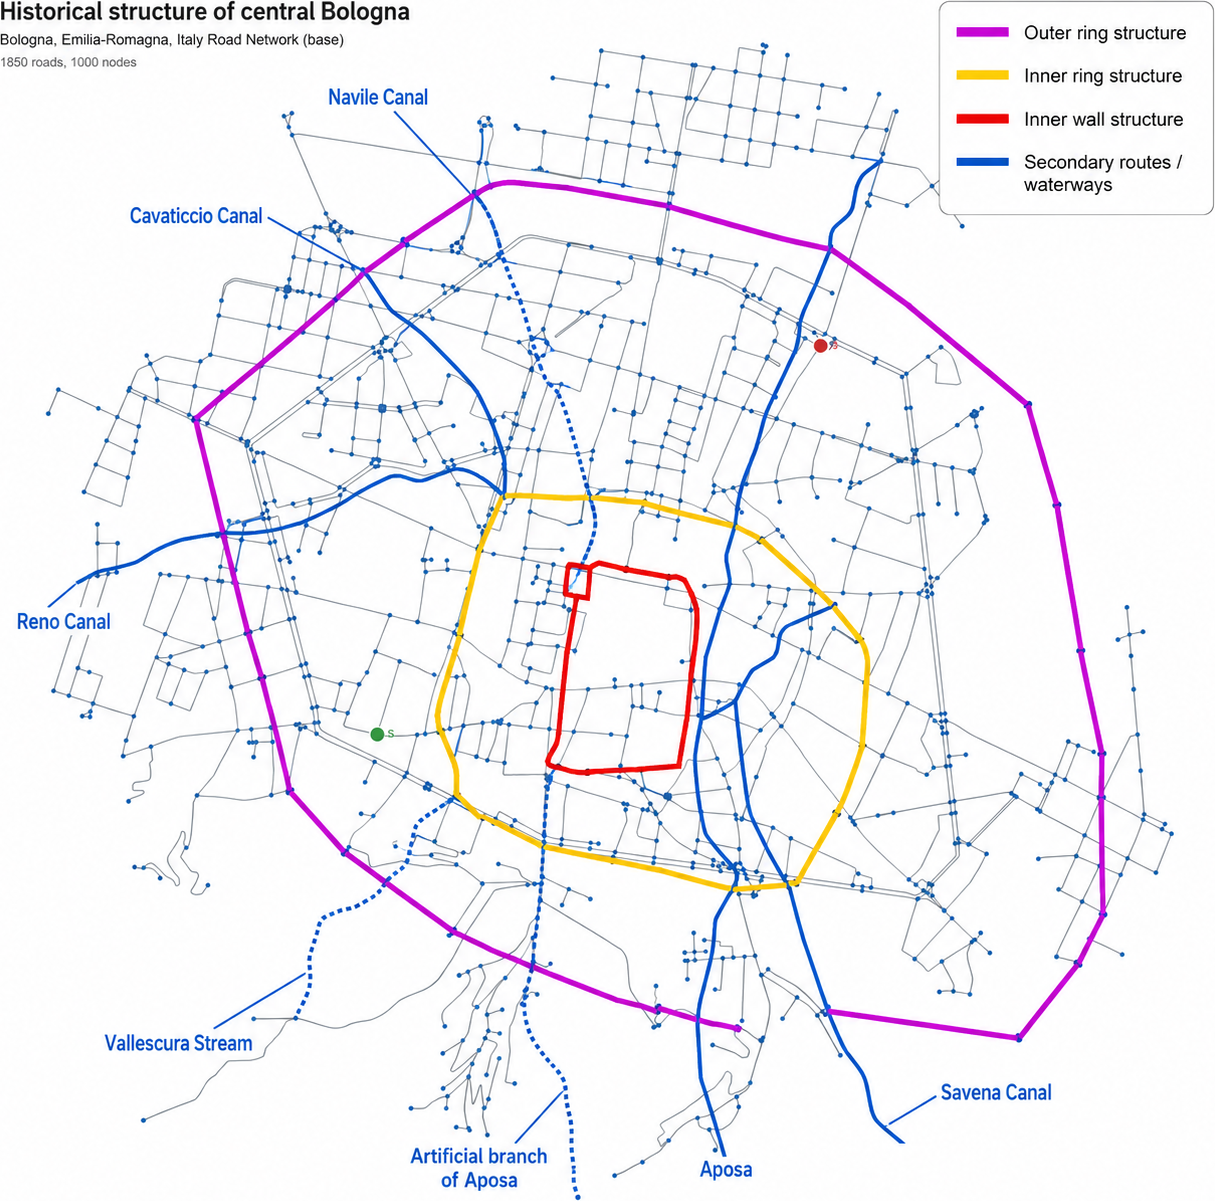
\includegraphics[height=0.69\textheight,width=\linewidth,keepaspectratio]{figures/bologna.png}
			\end{column}
		\end{columns}
	\end{frame}
	
	%% 3 --------------------------------------------------------------------------
	\begin{frame}{Why PDDL+ and not just a shortest-path search}
	\begin{columns}[c,onlytextwidth]
	\begin{column}{0.33\textwidth}
	{
	\setbeamercolor{block title}{bg=rRed,fg=white}
	\setbeamercolor{block body}{bg=rRed!7,fg=rInk}
	\begin{block}{A* / Dijkstra\hfill\textbf{\large$\times$}}
	\begin{itemize}
	\item specialised in finding the shortest path;
	\item need fixed, known road costs;
	\item extra real-world behaviour must be added
	outside the search.
	\end{itemize}
	\end{block}
	}
	\end{column}
	\hfill
	\begin{column}{0.62\textwidth}
	\begin{center}
	\colorbox{rPrimary}{\textcolor{white}{\bfseries\ \ PDDL+\ \ }}
	\end{center}
	\vspace{0.3em}
	\begin{columns}[T,onlytextwidth]
	\begin{column}{0.31\textwidth}
	\begin{block}{Actions}
	The decisions the planner makes: which road to drive next, and when to stop and refuel.
	\end{block}
	\end{column}
	\begin{column}{0.31\textwidth}
	\begin{alertblock}{Processes}
	Track what changes on its own while driving: time keeps passing and fuel keeps dropping as the vehicle moves.
	\end{alertblock}
	\end{column}
	\begin{column}{0.31\textwidth}
	\begin{exampleblock}{Events}
	Arriving at a junction, waiting at red lights, and moving to the next time window as time passes
	\end{exampleblock}
	\end{column}
	\end{columns}
	\end{column}
	\end{columns}
	\vspace{0.3cm}
	\takeaway{The domain is not static: one configuration file decides which features are compiled into it.}
	\end{frame}
	
	%% 4 --------------------------------------------------------------------------
	\begingroup
	\begin{frame}{The pipeline and the three research questions}
	\vspace{0.3cm}
	\centering

	{\small\color{rMuted}From a real city map to a plan validated in simulation.}

	\vspace{0.45cm}
	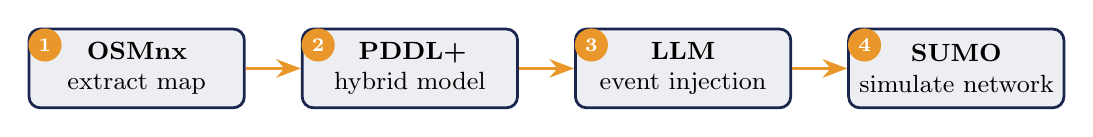
\begin{tikzpicture}[
	>=Stealth,
	node distance=7mm,
	st/.style={
		draw=rPrimary, fill=rPrimary!8, line width=1pt, rounded corners=4pt,
		minimum height=1.0cm, text width=2.5cm, align=center, font=\small
	},
	num/.style={
		circle, fill=rAccent, text=white, font=\bfseries\scriptsize,
		inner sep=1.2pt, minimum size=4.2mm
	}
	]
	\node[st] (a) {\textbf{OSMnx}\\extract map};
	\node[st,right=of a] (b) {\textbf{PDDL+}\\hybrid model};
	\node[st,right=of b] (c) {\textbf{LLM}\\event injection};
	\node[st,right=of c] (d) {\textbf{SUMO}\\simulate network};

	\foreach \n/\i in {a/1,b/2,c/3,d/4}
	\node[num] at ([shift={(2.2mm,-2.2mm)}]\n.north west) {\i};

	\foreach \x/\y in {a/b,b/c,c/d}
	\draw[->,rAccent,line width=1.3pt] (\x) -- (\y);
	\end{tikzpicture}

	\vspace{0.9cm}
	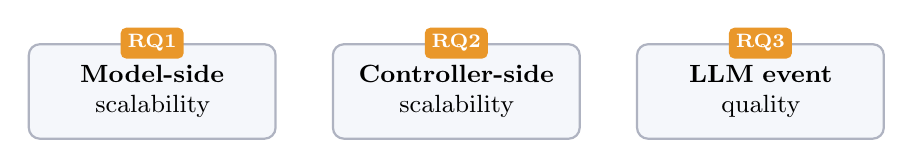
\begin{tikzpicture}[
	rq/.style={
		draw=rPrimary!35, fill=rBg, line width=0.8pt, rounded corners=4pt,
		minimum height=1.2cm, text width=2.9cm, align=center, font=\small
	},
	badge/.style={
		rounded corners=2pt, fill=rAccent, text=white,
		font=\bfseries\scriptsize, inner sep=2.5pt
	}
	]
	\node[rq] (r1) {\textbf{Model-side}\\scalability};
	\node[rq,right=7mm of r1] (r2) {\textbf{Controller-side}\\scalability};
	\node[rq,right=7mm of r2] (r3) {\textbf{LLM event}\\quality};

	\foreach \n/\i in {r1/RQ1,r2/RQ2,r3/RQ3}
	\node[badge] at (\n.north) {\i};
	\end{tikzpicture}

	\vspace{0.5cm}
	\takeaway{Three questions, three different bottlenecks: the model, the solving strategy, and the realism of the tests.}
	\end{frame}
	\endgroup
	
	%% 5 --------------------------------------------------------------------------
	\sectionframe{Foundation}{Realistic Features}{The three real-world features in our model: traffic lights, congestion, and fuel}
	
	%% 6 --------------------------------------------------------------------------
	\begin{frame}{Traffic lights}
		\begin{columns}[T,onlytextwidth]
			\begin{column}{0.65\textwidth}
				\begin{itemize}
					\item Each signal is graded \textbf{simple / medium / complex} from its number of approaches and its highest incident road class.
					\item Green / yellow / red are \textbf{sampled per signal} from configurable ranges (defaults 20--30\,/\,3--6\,/\,20--30\,s); complex junctions draw longer phases.
					\item On arrival, the expected wait for uniform arrivals is added:
				\end{itemize}
				\[
				d=\frac{r^{2}}{2\,C},\qquad C=g+y+r .
				\]
				\begin{center}
				{\scriptsize Uniform-delay term of Webster's delay model (1958), for undersaturated signals.}
				\end{center}
			\end{column}
			\begin{column}{0.35\textwidth}
				\centering
				
\begin{tikzpicture}
					\draw[rounded corners=3pt,fill=rInk] (0,0) rectangle (1.15,3.1);
					\fill[red!80!black] (0.575,2.55) circle (0.34);
					\fill[yellow!85!black] (0.575,1.55) circle (0.34);
					\fill[rTeal] (0.575,0.55) circle (0.34);
				\end{tikzpicture}
			\end{column}
		\end{columns}
		\vspace{0.5em}
		\takeaway{Only signalized nodes cost time, and that cost grows with the junction's complexity and the red share of its cycle.}
	\end{frame}
	
	%% 7 --------------------------------------------------------------------------
	\begin{frame}{Congestion}
	Simulated background routes determine how many vehicles use each road; that load sets the slowdown.
	\vfill
	\begin{columns}[c,onlytextwidth]
	\begin{column}{0.57\textwidth}
	\[
		\text{factor}=\min\!\Big(f_{\max},\;1+\tfrac{\text{load}}{\text{max-load}}\,(f_{\max}-1)\Big)
	\]
	\vspace{-0.5em}
	\begin{center}
		{\footnotesize\color{rMuted}\textbf{\(f_{\max}\)}: max congestion factor.}
	\end{center}
	\vspace{1.4em}
	\[
		\text{effective speed}=\frac{\text{speed limit}}{\text{factor}}
	\]
	\vspace{1.4em}
	\[
		\text{road time}=\frac{\text{length}}{\text{effective speed}}
	\]
	\end{column}
	\hfill
	\begin{column}{0.38\textwidth}
	\centering
	\renewcommand{\arraystretch}{1.35}
	\begin{tabular}{@{}l@{\hskip 1.2em}c@{}}
	\toprule
	\rowcolor{rPrimary!12}\textbf{Road class} & \textbf{Max-load (veh.)}\\
	\midrule
	Local & 20\\
	Arterial & 35\\
	Major & 50\\
	\bottomrule
	\end{tabular}
	\end{column}
	\end{columns}
	\vfill
	\end{frame}
	

  \begin{frame}[fragile]{Static vs.\ dynamic congestion}
  Congestion enters the plan as a cost per road. The only question is whether that cost may change over time.

  \begin{columns}[T,onlytextwidth]
    \begin{column}{0.48\textwidth}
      \begin{block}{Static congestion}
  \begin{lstlisting}
(:action start-traversal
 :parameters (?v ?r ?from ?to)
 :effect (assign (speed ?v)
   (/ (speed-limit ?r) (congestion-factor ?r))))

;; one value per road
(= (congestion-factor macro_0002) 1.54)
\end{lstlisting}
      {\scriptsize The factor is divided at plan time: one value per road, \(|R|\).}
    \end{block}
	{\small Later we will cover the \textbf{hybrid} congestion}
  \end{column}
    \hfill
    \begin{column}{0.48\textwidth}
      \begin{exampleblock}{Dynamic congestion --- one window}
  \begin{lstlisting}
(:action start-traversal-dynamic
 :parameters (?v ?r ?from ?to ?w)
 :precondition (and (dynamic-road ?r) (current-window ?w))
 :effect (assign (speed ?v) (effective-speed-window ?r ?w)))

;; one value per road per window
(current-window tw_00000)
(= (effective-speed-window macro_0000 tw_00000) 8.09)
\end{lstlisting}
      {\scriptsize An \texttt{advance-window} event moves the window on: one value per road \emph{and} window, \(|R|\times|W|\).}
      \end{exampleblock}
    \end{column}
  \end{columns}
  \vfill
  \takeaway{With one window the two coincide; every extra window multiplies the numeric facts.}
  \note{Time: 40 seconds. Follow Figure 2 of the report. Static congestion fixes one factor and one duration per road for the whole plan. Dynamic congestion stores one duration per road and per window, and a single global event advances the active window. Showing one window makes the mechanism readable, because it is exactly the static case plus the window index. This sets up the dynamic congestion section.}
  \end{frame}

	%% 8 --------------------------------------------------------------------------
	\begin{frame}{Fuel}
		\textbf{Constraint:} a road can be entered only with enough fuel to cross it,
		\(\;\text{fuel}\ge\text{length}\times\text{rate}\;\).
		\vspace{0.05cm}
		\begin{columns}[T,onlytextwidth]
			\begin{column}{0.45\textwidth}
				\begin{block}{Discrete cost}
					One drop when the road is taken:
					\[ \Delta f=-\,\text{length}\times\text{rate} \]
					More efficient, but less realistic.
				\end{block}
			\end{column}
			\begin{column}{0.45\textwidth}
				\begin{exampleblock}{Continuous process}
					Fuel burns while moving:
					\[ \frac{df}{dt}=-\,\text{speed}\times\text{rate} \]
					More realistic, but less efficient.
				\end{exampleblock}
			\end{column}
		\end{columns}
		\vspace{0.25cm}
		{\small Stations can be real fuel points or a seeded random
			subset of nodes.}
		\vspace{0.5em}
		\takeaway{Refuelling is \emph{instantaneous} for the planner (it just fills the tank).}
		\note{Time: 45 seconds. Explain the hard fuel precondition before entering a road. Contrast the discrete model, where the resource changes once per traversal, with the continuous process model. Fuel stations are either real OSM amenities or a reproducible seeded fallback.}
	\end{frame}
	
	%% 9 --------------------------------------------------------------------------
	\begin{frame}[plain]
		\begin{tikzpicture}[remember picture,overlay]
			\fill[rPrimary](current page.south west) rectangle (current page.north east);
			\fill[rAccent]([yshift=-3mm]current page.west) rectangle ([yshift=0mm]current page.east);
			\node[anchor=west,text=rAccent,font=\Large\bfseries]
			at ([xshift=13mm,yshift=24mm]current page.west) {RQ1};
			\node[anchor=west,text=white,font=\huge\bfseries,text width=0.82\paperwidth]
			at ([xshift=13mm,yshift=7mm]current page.west) {Model-side Scalability};
			\node[anchor=north west,text=rBg,font=\small,text width=0.40\paperwidth]
			at ([xshift=13mm,yshift=-18mm]current page.west)
			{How can we reduce what ENHSP must\\represent and ground?};
			
			\node[
				anchor=north east,
				fill=rSecondary!58,
				draw=white!30,
				line width=0.8pt,
				rounded corners=4pt,
				inner sep=5pt,
				text=white
			]
			at ([xshift=-13mm,yshift=-12mm]current page.east)
			{\begin{minipage}{0.29\paperwidth}
				{\small\bfseries\textcolor{rAccent}{Reference case}}\par
				\vspace{0.8mm}
				{\bfseries \(L=500\quad R=862\)}\par
				\vspace{0.7mm}
				{\tiny\color{rBg}\(L\): locations \qquad \(R\): roads}
			\end{minipage}};
		\end{tikzpicture}
		\note{Time: 15 seconds. State RQ1: the first strategy changes the planning model itself through selective detail, abstraction, reformulation, and compilation. Establish only the original Bologna reference network: 500 locations and 862 directed roads. The later slides introduce each reduction when it becomes relevant.}
	\end{frame}
	
	%% 10 -------------------------------------------------------------------------
	\begin{frame}{Hybrid congestion}
		\begin{columns}[T,onlytextwidth]
			\begin{column}{0.43\textwidth}
				{\small Hybrid selection compares each road's congestion factor across all windows. A road remains dynamic only when}
				\vspace{-0.05cm}
				\[
				\max_w c_{r,w}-\min_w c_{r,w}\geq\theta .
				\]
				{\scriptsize \(c_{r,w}\) is the congestion factor of road \(r\) in window \(w\).}
			\end{column}
			\begin{column}{0.54\textwidth}
				\centering
				{\scriptsize\bfseries Threshold calibration on the reference case\par}
				\vspace{0.04cm}
				\renewcommand{\arraystretch}{1.12}
				\setlength{\tabcolsep}{3.4pt}
				\begin{tabular}{@{}c r r@{}}
					\toprule
					\(\theta\) & Dynamic roads & Road--window values\\
					\midrule
					0.05 & 390 & 8,580\\
					0.07 & 54 & 1,134\\
					\rowcolor{rRed!13}
					\textcolor{rRed}{\bfseries 0.10} &
					\textcolor{rRed}{\bfseries 47} &
					\textcolor{rRed}{\bfseries 987}\\
					0.12 & 4 & 60\\
					\bottomrule
				\end{tabular}
			\end{column}
		\end{columns}
		
		\vspace{0.78cm}
		\begin{columns}[T,onlytextwidth]
			\begin{column}{0.48\textwidth}
				\metric{rAccent!16}{829 $\rightarrow$ 47}{roads kept dynamic}
			\end{column}
			\begin{column}{0.48\textwidth}
				\metric{rTeal!14}{17,409 $\rightarrow$ 47 $\times$ 21 $\rightarrow$ 987}{dynamic road--window values}
			\end{column}
		\end{columns}
		\vfill
		\takeaway{Hybrid congestion reduces temporal detail by \(94.3\%\) in the 500-node reference case.}
		\note{Time: 65 seconds. Clarify that this is the hybrid-selection rule, not the congestion-factor formula shown earlier. The table uses the same 500-node Bologna reference artifacts as the rest of the slide. At 0.05, 390 roads remain dynamic and create 8,580 road-window values; at 0.07, 54 roads create 1,134 values; at 0.10, 47 roads create 987 values; and at 0.12 only four roads and 60 values remain. The highlighted 0.10 row is the selected balance. With 21 selected global windows, the final reduction is from 17,409 to 47 times 21, or 987 values.}
	\end{frame}
	
	%% 11 -------------------------------------------------------------------------
	\begin{frame}{Macro-road abstraction}
		\begin{columns}[T,onlytextwidth]
			\begin{column}{0.22\textwidth}
				\renewcommand{\arraystretch}{1.36}
				\setlength{\tabcolsep}{2pt}
				\small
				\vspace{0.5cm}
				\begin{tabular}{@{}l@{}}
					\toprule
					\textbf{Protected elements}\\
					\midrule
					Start / goal\\
					Traffic light\\
					Fuel station\\
					Branch node\\
					Road class / speed\\
					\bottomrule
				\end{tabular}
			\end{column}
			\begin{column}{0.75\textwidth}
				\centering
				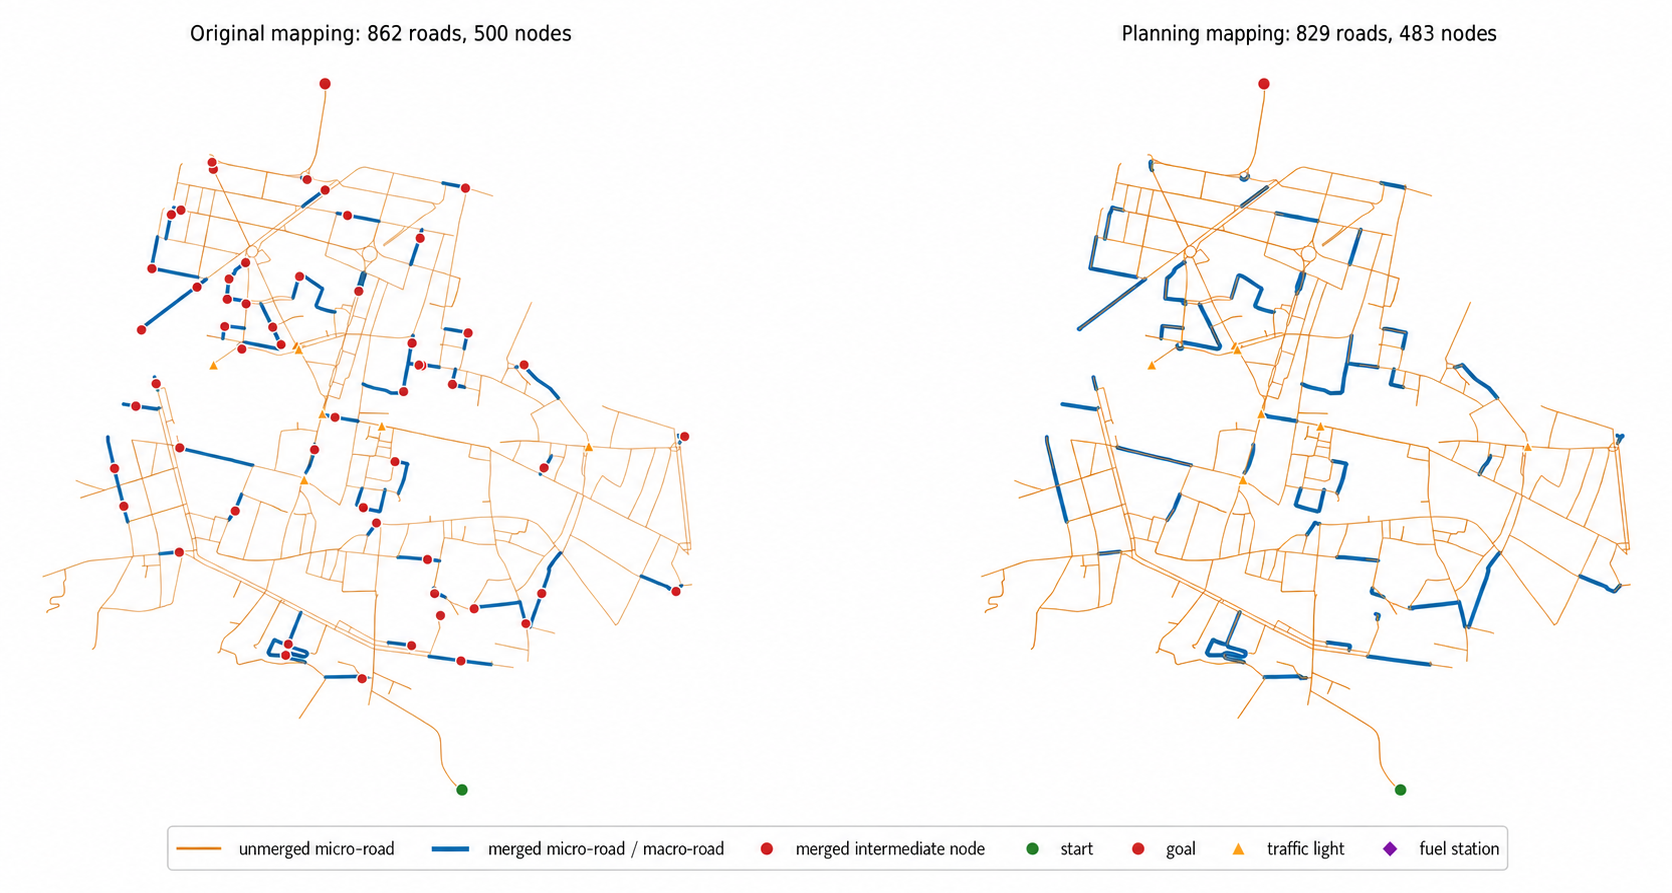
\includegraphics[height=0.59\textheight,width=\linewidth,keepaspectratio]{figures/macro_roads_comparison.png}
			\end{column}
		\end{columns}
		
		\vfill
		\begin{columns}[T,onlytextwidth]
			\begin{column}{0.48\textwidth}
				\metric{rPrimary!10}{500 $\rightarrow$ 483}{locations}
			\end{column}
			\begin{column}{0.48\textwidth}
				\metric{rAccent!14}{862 $\rightarrow$ 829}{roads}
			\end{column}
		\end{columns}
		\note{Time: 50 seconds. Explain orally that only linear chains without a planning decision can be compressed. Start and goal, traffic lights, fuel stations, and branch nodes remain explicit. Adjacent segments also stop merging when road class or speed is incompatible. Read the before-and-after values from the fixed 500-node case.}
	\end{frame}
	
	%% 12 -------------------------------------------------------------------------
	\begin{frame}{Configurations}
		{\small\bfseries Three independent axes\par}
		\vspace{0.08cm}
		\renewcommand{\arraystretch}{1.14}
		\setlength{\tabcolsep}{4pt}
		\scriptsize
		\begin{tabularx}{\linewidth}{@{}>{\bfseries}p{2.05cm} X >{\raggedright\arraybackslash}p{5.35cm}@{}}
			\toprule
			Axis & Question & Choices\\
			\midrule
			Traversal & How does the vehicle cross a road? &
			\texttt{process} / \texttt{compiled\_duration}\\
			State & Where is the vehicle state represented? &
			\texttt{node\_based} / \texttt{line\_graph}\\
			Generation & Who instantiates the valid movements? &
			ENHSP (\texttt{parameterized}) / Python (\texttt{compiled})\\
			\bottomrule
		\end{tabularx}
		
		\vfill
		\centering
		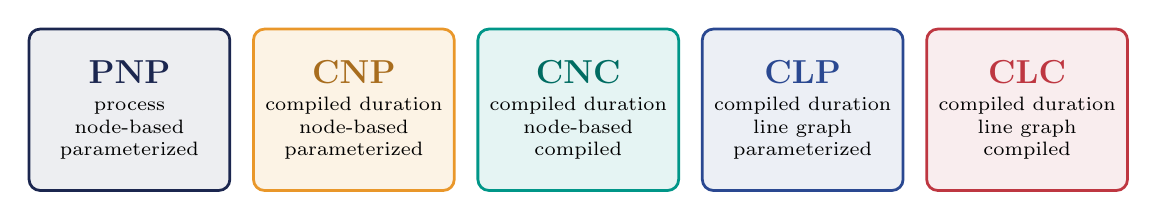
\begin{tikzpicture}[
			modelbox/.style={
				rounded corners=4pt,
				minimum width=2.55cm,
				minimum height=2.05cm,
				text width=2.25cm,
				align=center,
				inner sep=4pt,
				font=\scriptsize,
				line width=1pt
			}
			]
			\node[modelbox,draw=cPNP,fill=cPNP!8] at (0,0) {
				{\large\bfseries\color{cPNP}PNP}\\[2pt]
				process\\node-based\\parameterized
			};
			\node[modelbox,draw=cCNP,fill=cCNP!12] at (2.85,0) {
				{\large\bfseries\color{cCNP!72!black}CNP}\\[2pt]
				compiled duration\\node-based\\parameterized
			};
			\node[modelbox,draw=cCNC,fill=cCNC!10] at (5.70,0) {
				{\large\bfseries\color{cCNC!72!black}CNC}\\[2pt]
				compiled duration\\node-based\\compiled
			};
			\node[modelbox,draw=cCLP,fill=cCLP!9] at (8.55,0) {
				{\large\bfseries\color{cCLP}CLP}\\[2pt]
				compiled duration\\line graph\\parameterized
			};
			\node[modelbox,draw=cCLC,fill=cCLC!9] at (11.40,0) {
				{\large\bfseries\color{cCLC}CLC}\\[2pt]
				compiled duration\\line graph\\compiled
			};
		\end{tikzpicture}
		\note{Time: 65 seconds. First explain the three questions. Traversal asks how a road crossing is represented. State asks whether the vehicle is attached to a node or to an edge. Generation asks whether ENHSP or Python instantiates valid moves. Then decode the five configurations and introduce their stable colours, which remain unchanged in the grounding and result slides.}
	\end{frame}
	
	%% 13 -------------------------------------------------------------------------
	\begin{frame}[fragile]{Traversal and state representation}
		\setbeamerfont{block title}{size=\small}
		\noindent{\small\bfseries Traversal: process vs compiled duration\par}
		\vspace{-0.20cm}
		\begin{columns}[T,onlytextwidth]
			\begin{column}{0.48\textwidth}
				\setbeamercolor{block title}{bg=cPNP,fg=white}
				\setbeamercolor{block body}{bg=cPNP!6,fg=rInk}
				\begin{block}{Process \hfill \textnormal{PNP}}
\begin{lstlisting}[basicstyle=\ttfamily\scriptsize]
(:action start-traversal
 :effect (moving ?v))
(:process traverse
 :effect (decrease (remaining ?v)
   (* #t (speed ?v))))
(:event arrive
 :effect (at ?v ?to))
\end{lstlisting}
				\end{block}
			\end{column}
			\begin{column}{0.48\textwidth}
				\setbeamercolor{block title}{bg=cCNP,fg=white}
				\setbeamercolor{block body}{bg=cCNP!8,fg=rInk}
				\begin{block}{Compiled duration \hfill \textnormal{CNP}}
\begin{lstlisting}[basicstyle=\ttfamily\scriptsize]
(:action traverse-road
 :parameters (?v ?r ?from ?to)
 :precondition (and (at ?v ?from)
   (connects ?r ?from ?to))
 :effect (and (not (at ?v ?from))
   (at ?v ?to)
   (increase (travel-time ?v)
    (travel-duration ?r))))
\end{lstlisting}
				\end{block}
			\end{column}
		\end{columns}
		
		\vspace{0.08cm}
		\noindent{\small\bfseries State: node-based vs line graph\par}
		\vspace{-0.20cm}
		\begin{columns}[T,onlytextwidth]
			\begin{column}{0.48\textwidth}
				\setbeamercolor{block title}{bg=cCNP,fg=white}
				\setbeamercolor{block body}{bg=cCNP!7,fg=rInk}
				\begin{block}{Node-based \hfill \textnormal{\textcolor{white}{CNP / CNC}}}
\begin{lstlisting}[basicstyle=\ttfamily\scriptsize]
(:action traverse-road
 :parameters (?v ?r ?from ?to)
 :precondition (and (at ?v ?from)
   (connects ?r ?from ?to))
 :effect (at ?v ?to))
\end{lstlisting}
				\end{block}
			\end{column}
			\begin{column}{0.48\textwidth}
				\setbeamercolor{block title}{bg=cCLP,fg=white}
				\setbeamercolor{block body}{bg=cCLP!7,fg=rInk}
				\begin{block}{Line graph \hfill \textnormal{\textcolor{white}{CLP / CLC}}}
\begin{lstlisting}[basicstyle=\ttfamily\scriptsize]
(:action traverse-road
 :parameters (?v ?r ?next)
 :precondition (and (ready-road ?v ?r)
   (road-next ?r ?next))
 :effect (ready-road ?v ?next))
\end{lstlisting}
				\end{block}
			\end{column}
		\end{columns}
		\note{Time: 75 seconds. Read the slide by rows. The upper row compares traversal semantics: the process baseline separates start, continuous movement, and arrival, while compiled duration uses one numeric action. The lower row compares state representation: node-based actions expose a road and two endpoints; the line graph exposes only a current road and a valid successor. The next slide isolates the action-generation choice, which is where singleton types remove the largest grounding burden.}
	\end{frame}
	
	%% 14 -------------------------------------------------------------------------
	\begin{frame}[fragile]{Action generation: singleton types}

	\vspace{-0.5cm}
		\begin{columns}[T,onlytextwidth]
			\begin{column}{0.48\textwidth}
				\setbeamercolor{block title}{bg=rPrimary,fg=white}
				\setbeamercolor{block body}{bg=rPrimary!6,fg=rInk}
				\begin{block}{Parameterized \hfill \textnormal{PNP / CNP / CLP}}
\begin{lstlisting}[basicstyle=\ttfamily\scriptsize]
(:action traverse-road
 :parameters
  (?v - vehicle
   ?r - road
   ?from ?to - location)
 :precondition (and
  (at ?v ?from)
  (connects ?r ?from ?to))
 :effect (and
  (not (at ?v ?from))
  (at ?v ?to)))
\end{lstlisting}
				\end{block}
				{\scriptsize\textbf{ENHSP:} one generic schema is grounded over
					every type-compatible road/location tuple, then invalid
					combinations are filtered.}
			\end{column}
			\begin{column}{0.48\textwidth}
				\setbeamercolor{block title}{bg=cCNC,fg=white}
				\setbeamercolor{block body}{bg=cCNC!7,fg=rInk}
				\begin{block}{Compiled singleton types \hfill \textnormal{CNC / CLC}}
\begin{lstlisting}[basicstyle=\ttfamily\scriptsize]
(:types
 loc_a_t loc_b_t - location
 road_0001_t - road)
(:objects
 loc_a - loc_a_t
 loc_b - loc_b_t
 road_0001 - road_0001_t)
(:action traverse-road-static-road_0001
 :parameters (?v - vehicle
  ?r - road_0001_t
  ?from - loc_a_t ?to - loc_b_t)
 :precondition (and (at ?v ?from)
  (road-open ?r)) ...)
\end{lstlisting}
				\end{block}
				{\scriptsize\textbf{Python:} one schema is emitted per valid
					transition; each singleton type admits exactly one object.}
			\end{column}
		\end{columns}
		\vfill
		\takeaway{Singleton types move valid action instantiation from ENHSP to Python.}
		\note{Time: 80 seconds. This is the central generation-axis optimization. On the left, the parameterized schema accepts every object of the broad road and location types, so ENHSP constructs their cross product and later checks the topology. On the right, Python first identifies one valid transition, creates a singleton subtype for each participating object, and emits a specialized action. Since each subtype contains exactly one object, each PDDL parameter has a single legal binding and invalid combinations never reach the grounder.}
	\end{frame}
	
		%% 15 -------------------------------------------------------------------------
	\begin{frame}{Grounding: exposure vs retained structures}
		\centering
		{\small\textbf{500-node hybrid reference after macro preprocessing}\par}
		\vspace{0.05cm}
		{\scriptsize
			Road level: \(R=829\), \(L=483\), \(W=21\), \(S=782\), \(D=47\).\\
			Line graph: \(T_s=1{,}471\) valid static transitions;
			\(T_d=79\) valid dynamic transitions.}
		
		\vspace{0.12cm}
		{\scriptsize
			\textbf{Candidates}: loose assignments exposed to ENHSP
			\qquad
			\textbf{Retained (derived)}: valid mechanisms after static filtering\par}
		
		\vspace{0.12cm}
		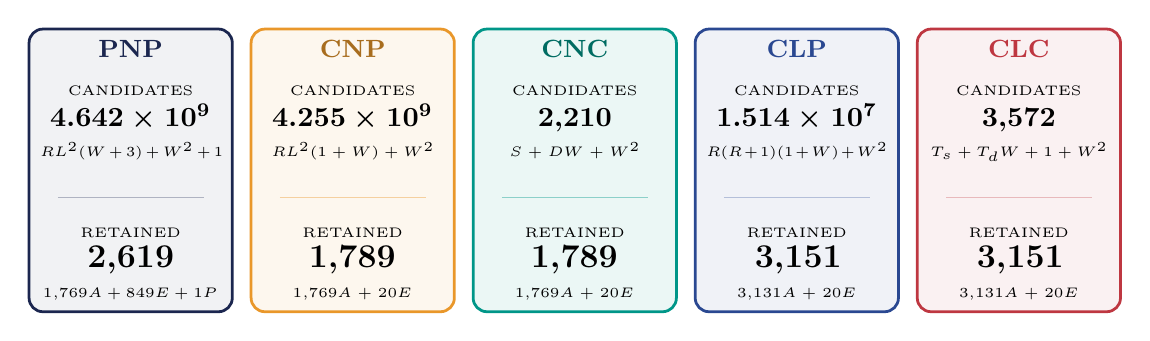
\begin{tikzpicture}[
			n/.style={
				rounded corners=5pt,
				minimum width=2.58cm,
				minimum height=3.18cm,
				text width=2.30cm,
				align=center,
				inner sep=4pt,
				line width=1pt
			}
			]
			\node[n,draw=cPNP,fill=cPNP!6](a) at (0,0) {
				{\small\textcolor{cPNP}{\bfseries PNP}}\\[2pt]
				{\tiny CANDIDATES}\\[-1pt]
				{\normalsize\bfseries\boldmath \(4.642\times10^9\)}\\[-1pt]
				{\tiny \(RL^2(W+3)+W^2+1\)}\\[3pt]
				{\color{cPNP!35}\rule{1.85cm}{0.4pt}}\\[2pt]
				{\tiny RETAINED}\\[-1pt]
				{\large\bfseries 2,619}\\[-1pt]
				{\tiny \(1{,}769A+849E+1P\)}
			};
			\node[n,draw=cCNP,fill=cCNP!8](b) at (2.82,0) {
				{\small\textcolor{cCNP!72!black}{\bfseries CNP}}\\[2pt]
				{\tiny CANDIDATES}\\[-1pt]
				{\normalsize\bfseries\boldmath \(4.255\times10^9\)}\\[-1pt]
				{\tiny \(RL^2(1+W)+W^2\)}\\[3pt]
				{\color{cCNP!45}\rule{1.85cm}{0.4pt}}\\[2pt]
				{\tiny RETAINED}\\[-1pt]
				{\large\bfseries 1,789}\\[-1pt]
				{\tiny \(1{,}769A+20E\)}
			};
			\node[n,draw=cCNC,fill=cCNC!8](c) at (5.64,0) {
				{\small\textcolor{cCNC!72!black}{\bfseries CNC}}\\[2pt]
				{\tiny CANDIDATES}\\[-1pt]
				{\normalsize\bfseries 2,210}\\[-1pt]
				{\tiny \(S+DW+W^2\)}\\[3pt]
				{\color{cCNC!45}\rule{1.85cm}{0.4pt}}\\[2pt]
				{\tiny RETAINED}\\[-1pt]
				{\large\bfseries 1,789}\\[-1pt]
				{\tiny \(1{,}769A+20E\)}
			};
			\node[n,draw=cCLP,fill=cCLP!7](d) at (8.46,0) {
				{\small\textcolor{cCLP}{\bfseries CLP}}\\[2pt]
				{\tiny CANDIDATES}\\[-1pt]
				{\normalsize\bfseries\boldmath \(1.514\times10^7\)}\\[-1pt]
				{\tiny \(R(R+1)(1+W)+W^2\)}\\[3pt]
				{\color{cCLP!35}\rule{1.85cm}{0.4pt}}\\[2pt]
				{\tiny RETAINED}\\[-1pt]
				{\large\bfseries 3,151}\\[-1pt]
				{\tiny \(3{,}131A+20E\)}
			};
			\node[n,draw=cCLC,fill=cCLC!7](e) at (11.28,0) {
				{\small\textcolor{cCLC}{\bfseries CLC}}\\[2pt]
				{\tiny CANDIDATES}\\[-1pt]
				{\normalsize\bfseries 3,572}\\[-1pt]
				{\tiny \(T_s+T_dW+1+W^2\)}\\[3pt]
				{\color{cCLC!35}\rule{1.85cm}{0.4pt}}\\[2pt]
				{\tiny RETAINED}\\[-1pt]
				{\large\bfseries 3,151}\\[-1pt]
				{\tiny \(3{,}131A+20E\)}
			};
		\end{tikzpicture}
		
		\vspace{-0.02cm}
		{\scriptsize \(A=\) action \qquad \(E=\) event \qquad \(P=\) process\par}
		\vfill
		\takeaway{Grounding time depends on both candidate exposure and retained structures.}
		\note{Time: 75 seconds. This slide separates two quantities that must not be conflated. Candidate exposure is a loose type-based Cartesian upper bound, not an exact count of ENHSP operations. Retained structures are derived from the static topology of the 500-node hybrid reference case; the parameterized runs did not complete at this scale, so these are not measured ENHSP output counts. For PNP, the candidate formula contains static and dynamic start actions, \(RL^2(1+W)\); two arrival-event schemas, \(2RL^2\); the window-advance event, \(W^2\); and one vehicle process. After static filtering, PNP retains 1,769 start actions, 829 arrival events, 20 window-advance events, and one process. CNP removes the arrival events and process: its compiled traversal actions directly increase sim-time, while the window-advance event remains. The line graph reduces loose exposure but retains more actions because one road can have several successors. CNC and CLC reach the same retained structures as their parameterized counterparts while moving almost all instantiation to Python.}
	\end{frame}
	
	%% 16 -------------------------------------------------------------------------
	\begin{frame}{Which configuration is fastest on the same instance?}
		\begin{tikzpicture}[remember picture,overlay]
			\node[
			anchor=north east,
			rounded corners=3pt,
			draw=rPrimary!35,
			fill=rPrimary!8,
			inner xsep=7pt,
			inner ysep=3pt,
			font=\small\bfseries,
			text=rPrimary
			] at ([xshift=-0.55cm,yshift=-0.52cm]current page.north east) {300 nodes};
		\end{tikzpicture}
		\vspace{0.2cm}
		{\small All five configurations use the same map, start/goal, traffic,
			static congestion, and 8 GB ENHSP heap.\par}
		
		
		\begin{columns}[T,onlytextwidth]
			\begin{column}{0.71\textwidth}
				\centering
				{\scriptsize\textbf{Dark}: grounding \qquad \textbf{Light}: total planning\par}
				\vspace{-0.08cm}
				\begin{tikzpicture}
					\begin{axis}[
						width=\linewidth,
						height=0.49\textheight,
						ybar,
						ymode=log,
						ymin=0.7,
						ymax=260,
						ylabel={seconds (log scale)},
						symbolic x coords={PNP,CNP,CNC,CLP,CLC},
						xtick={PNP,CNP,CNC,CLP,CLC},
						tick label style={font=\scriptsize},
						label style={font=\scriptsize},
						grid=major,
						major grid style={draw=rLine},
						axis line style={draw=rMuted},
						enlarge x limits=0.15
						]
						\addplot[ybar,bar width=5pt,bar shift=-3pt,fill=cPNP,draw=cPNP] coordinates {(PNP,79.253)};
						\addplot[ybar,bar width=5pt,bar shift=3pt,fill=cPNP!28,draw=cPNP] coordinates {(PNP,146.901)};
						\addplot[ybar,bar width=5pt,bar shift=-3pt,fill=cCNP,draw=cCNP!72!black] coordinates {(CNP,40.379)};
						\addplot[ybar,bar width=5pt,bar shift=3pt,fill=cCNP!28,draw=cCNP!72!black] coordinates {(CNP,41.427)};
						\addplot[ybar,bar width=5pt,bar shift=-3pt,fill=cCNC,draw=cCNC!72!black] coordinates {(CNC,1.063)};
						\addplot[ybar,bar width=5pt,bar shift=3pt,fill=cCNC!25,draw=cCNC!72!black] coordinates {(CNC,2.542)};
						\addplot[ybar,bar width=5pt,bar shift=-3pt,fill=cCLP,draw=cCLP] coordinates {(CLP,76.263)};
						\addplot[ybar,bar width=5pt,bar shift=3pt,fill=cCLP!25,draw=cCLP] coordinates {(CLP,77.464)};
						\addplot[ybar,bar width=5pt,bar shift=-3pt,fill=cCLC,draw=cCLC] coordinates {(CLC,1.914)};
						\addplot[ybar,bar width=5pt,bar shift=3pt,fill=cCLC!25,draw=cCLC] coordinates {(CLC,3.606)};
					\end{axis}
				\end{tikzpicture}
			\end{column}
			\begin{column}{0.26\textwidth}
				\metric{cCNC!11}{38.0$\times$ / 16.3$\times$}{{\tiny grounding / planning speedup}}
				\vspace{0.55cm}
				\metric{cCLC!10}{39.8$\times$ / 21.5$\times$}{{\tiny grounding / planning speedup}}
				\vspace{0.10cm}
				\metric{cCNC!11}{3.605 s}{{\tiny grounding + planning}}
			\end{column}
		\end{columns}
		\vspace{0.12cm}
		
\begin{tikzpicture}
			\node[
				rounded corners=3pt,
				draw=rPrimary!28,
				fill=rPrimary!4,
				text width=0.94\textwidth,
				align=center,
				inner xsep=7pt,
				inner ysep=4pt
			] {
				{\scriptsize\textbf{Grounded structures on this static instance:}\quad
				\textcolor{cPNP}{\textbf{PNP}} \(925=462A+462E+1P\)
				\quad
				\textcolor{cCNP!72!black}{\textbf{CNP}}/\textcolor{cCNC!72!black}{\textbf{CNC}} \(462A\)
				\quad
				\textcolor{cCLP}{\textbf{CLP}}/\textcolor{cCLC}{\textbf{CLC}} \(851A\)}
			};
		\end{tikzpicture}
		\vfill
		\takeaway{Compilation removes mechanisms; singleton types remove generic grounding.}
		\note{Time: 75 seconds. This experiment fixes a 300-node static instance so all five configurations terminate successfully. The light bar is the total ENHSP planning call, including grounding and preprocessing, rather than pure search time. The grounded-structure strip explains the apparently conflicting results. PNP and CNP share the same dominant node-based action exposure, but PNP produces 462 actions, 462 arrival events, and one process, while CNP produces only 462 actions. CLP has lower parameter arity, yet road-to-road branching leaves 851 valid actions, so its grounding time is close to PNP and higher than CNP. CNC and CLC retain the same valid actions as CNP and CLP respectively, but singleton types prevent ENHSP from enumerating the generic Cartesian products. In the raw logs, heuristic and search times are only 13 and 42 ms for CNP, 17 and 53 ms for CNC, 13 and 83 ms for CLP, and 24 and 68 ms for CLC; their total-time differences are therefore dominated by grounding. PNP additionally requires 3.023 s of heuristic computation and 3.902 s of search because continuous process/event semantics remain.}
	\end{frame}
	
	%% 17 -------------------------------------------------------------------------
	\begin{frame}{How far can the two best configurations scale?}
		\textbf{\textcolor{cCNC!72!black}{CNC} and \textcolor{cCLC}{CLC} are carried forward from the fixed-instance comparison.}
		\vspace{0.16cm}
		\begin{columns}[T,onlytextwidth]
			\begin{column}{0.64\textwidth}
				\centering
				\begin{tikzpicture}
					\begin{axis}[
						width=\linewidth,
						height=0.54\textheight,
						xlabel={requested nodes},
						ylabel={planning time (s)},
						ymode=log,
						xmin=450,xmax=2050,
						ymin=6,ymax=700,
						xtick={500,1000,1500,2000},
						tick label style={font=\scriptsize},
						label style={font=\scriptsize},
						legend style={font=\scriptsize,at={(0.5,1.02)},anchor=south,legend columns=2,draw=none},
						grid=major,
						major grid style={draw=rLine},
						axis line style={draw=rMuted}
						]
						\addplot[very thick,cCNC,mark=*] coordinates {
							(500,8.431) (1000,33.011) (1500,89.963) (2000,245.256)
						};
						\addplot[very thick,cCLC,mark=square*] coordinates {
							(500,16.535) (1000,103.992) (1500,299.261) (2000,489.018)
						};
						\legend{CNC node-based,CLC line graph}
					\end{axis}
				\end{tikzpicture}
			\end{column}
			\begin{column}{0.33\textwidth}
				\centering\footnotesize
				\renewcommand{\arraystretch}{1.12}
				\setlength{\tabcolsep}{3.1pt}
				\begin{tabular}{@{}rrrr@{}}
					\toprule
					Nodes & Dyn. & Static & Win.\\
					\midrule
					500  & 47  & 782  & 21\\
					1000 & 78  & 1706 & 25\\
					1500 & 109 & 2629 & 25\\
					2000 & 110 & 3572 & 32\\
					\bottomrule
				\end{tabular}
				
				\vspace{0.28cm}
				\metric{cCNC!11}{245.3 s}{at 2,000 nodes}
				\vspace{0.30cm}
				\metric{cCLC!10}{489.0 s}{at 2,000 nodes}
			\end{column}
		\end{columns}
		\vfill
		\takeaway{Parameterized models already fail at 500 nodes (OOM); CNC and CLC reach 2,000.}
		\note{Time: 55 seconds. This second result asks how far the two best configurations from the previous experiment can scale. The parameterized alternatives already fail to complete at 500 nodes through memory exhaustion or timeout. Both compiled formulations scale from 500 to 2,000 requested nodes, and CNC remains faster at every size because a road can have several valid successor roads.}
	\end{frame}
	
	%% 17 -------------------------------------------------------------------------
	\begin{frame}[plain]
		\begin{tikzpicture}[remember picture,overlay]
			\fill[rPrimary](current page.south west) rectangle (current page.north east);
			\fill[rAccent]([yshift=-3mm]current page.west) rectangle ([yshift=0mm]current page.east);
			\node[anchor=west,text=rAccent,font=\Large\bfseries]
			at ([xshift=13mm,yshift=24mm]current page.west) {RQ2};
			\node[anchor=west,text=white,font=\huge\bfseries,text width=0.82\paperwidth]
			at ([xshift=13mm,yshift=7mm]current page.west) {Controller-side Scalability};
			\node[anchor=north west,text=rBg,font=\small,text width=0.40\paperwidth]
			at ([xshift=13mm,yshift=-18mm]current page.west)
			{Can we preserve the process model while\\reducing the horizon of each planner call?};

			\node[anchor=north east,fill=rSecondary!58,draw=white!30,line width=0.8pt,
			rounded corners=4pt,inner sep=5pt,text=white]
			at ([xshift=-13mm,yshift=-12mm]current page.east)
			{\begin{minipage}{0.29\paperwidth}
				{\small\bfseries\textcolor{rAccent}{Reference case}}\par
				\vspace{0.8mm}
				{\bfseries \(L=500\quad R=862\)}\par
				\vspace{0.7mm}
				{\tiny\color{rBg}model unchanged: process \(\cdot\) node-based \(\cdot\) parameterized}
			\end{minipage}};
		\end{tikzpicture}
		\note{Time: 10 seconds. RQ2 does not simplify the model: same 500-location, 862-road reference case, same process semantics. Only the control architecture changes.}
	\end{frame}
	
 
%% 18 --------------------------------------------------------------------------
\begin{frame}{A plan--act--replan loop replaces one monolithic solve}
	{\small Same \textbf{process $\cdot$ node-based $\cdot$ parameterized} model in every
		call --- only the \textbf{horizon} of each call shrinks.\par}
	\vspace{0.30cm}
	\begin{columns}[T,onlytextwidth]
		\begin{column}{0.30\textwidth}
			{\scriptsize\bfseries\color{rPrimary}ONE CALL\par}
			\vspace{0.10cm}
			
\begin{tikzpicture}
				\draw[rRed,fill=rRed!12,line width=0.8pt,rounded corners=2pt]
				(0,0) rectangle (3.75,0.52);
				\node[font=\tiny,text=rRed!70!black] at (1.875,0.26)
				{start $\longrightarrow$ goal};
			\end{tikzpicture}
			\par{\tiny\color{rMuted}grounding over the whole horizon\\
				$\Rightarrow$ \textcolor{rRed}{out of memory}\par}

			\vspace{0.42cm}
			{\scriptsize\bfseries\color{rPrimary}MANY SMALL CALLS\par}
			\vspace{0.10cm}
			
\begin{tikzpicture}
				\foreach \i in {0,1,2,3}{%
					\draw[rTeal,fill=rTeal!14,line width=0.8pt,rounded corners=2pt]
					(\i*0.95,0) rectangle (\i*0.95+0.78,0.52);
				}
			\end{tikzpicture}
			\par{\tiny\color{rMuted}each problem covers one window / leg\\
				$\Rightarrow$ grounding stays small\par}
		\end{column}
		\begin{column}{0.66\textwidth}
			\centering
			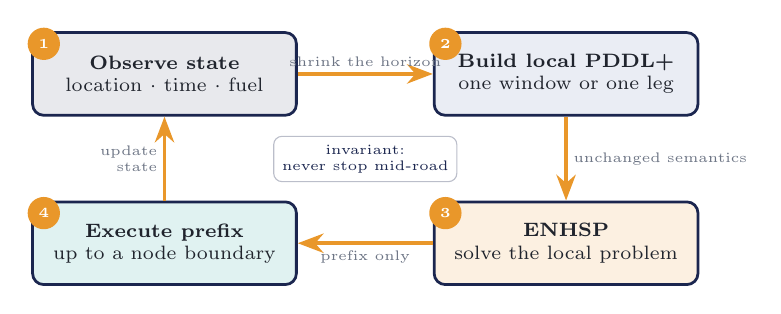
\begin{tikzpicture}[
				>=Stealth,
				n/.style={
					draw=rPrimary,line width=1pt,rounded corners=4pt,
					minimum width=3.35cm,minimum height=1.05cm,
					align=center,font=\scriptsize,text=rInk
				},
				lbl/.style={font=\tiny,text=rMuted,inner sep=2pt},
				badge/.style={
					circle,fill=rAccent,text=white,font=\tiny\bfseries,
					inner sep=1.2pt,minimum size=4.1mm
				}
				]
				\node[n,fill=rPrimary!10]   (s) at (0,2.15)   {\textbf{Observe state}\\location $\cdot$ time $\cdot$ fuel};
				\node[n,fill=rSecondary!10] (p) at (5.1,2.15) {\textbf{Build local PDDL+}\\one window or one leg};
				\node[n,fill=rAccent!14]    (e) at (5.1,0)    {\textbf{ENHSP}\\solve the local problem};
				\node[n,fill=rTeal!12]      (x) at (0,0)      {\textbf{Execute prefix}\\up to a node boundary};

				\draw[->,rAccent,line width=1.4pt] (s) -- node[lbl,above]{shrink the horizon} (p);
				\draw[->,rAccent,line width=1.4pt] (p) -- node[lbl,right]{unchanged semantics} (e);
				\draw[->,rAccent,line width=1.4pt] (e) -- node[lbl,below]{prefix only} (x);
				\draw[->,rAccent,line width=1.4pt] (x) -- node[lbl,left,align=right]{update\\state} (s);

				\node[badge] at ($(s.north west)+(0.16,-0.16)$) {1};
				\node[badge] at ($(p.north west)+(0.16,-0.16)$) {2};
				\node[badge] at ($(e.north west)+(0.16,-0.16)$) {3};
				\node[badge] at ($(x.north west)+(0.16,-0.16)$) {4};

				\node[draw=rPrimary!30,fill=white,rounded corners=3pt,
				inner sep=3pt,font=\tiny,text=rPrimary,align=center]
				at (2.55,1.07) {invariant:\\never stop mid-road};
			\end{tikzpicture}
		\end{column}
	\end{columns}
	\vfill
	\takeaway{The model stays rich; the controller makes each individual planning problem small.}
	\note{Time: 55 seconds. Contrast the two bars on the left first: a single monolithic call grounds the entire start-to-goal horizon, the controller grounds one window or one leg at a time. Then walk the loop clockwise and stress the invariant: execution always stops at a node, so the next local problem never has to invent a mid-road position.}
\end{frame}


%% 19 --------------------------------------------------------------------------
\begin{frame}{The congestion controller replans by time window}
	\begin{columns}[T,onlytextwidth]
		\begin{column}{0.36\textwidth}
			{\setbeamertemplate{itemize item}{\color{rInk}\scriptsize\(\bullet\)}
			\begin{block}{Decomposition by time}
				\small
				\begin{itemize}
					\item one snapshot per window
					\item goal never changes
					\item prefix stops at a node
					\item unchanged costs: reuse
				\end{itemize}
			\end{block}}
			\vspace{0.30cm}
			\metric{rTeal!14}{7 windows}{{\scriptsize reused from cache on the reference case}}
		\end{column}
		\begin{column}{0.62\textwidth}
			\centering
			\includegraphics[height=0.56\textheight,width=\linewidth,keepaspectratio]%
			{figures/congestion_controller.png}
			\par{\scriptsize\color{rMuted}Successive 30\,s congestion windows along the 500-node route.\par}
		\end{column}
	\end{columns}
	\vspace{0.30cm}
	\takeaway{Congestion stays dynamic \emph{across} windows; every single PDDL+ problem stays static.}
	\note{Time: 50 seconds. On the reference case the horizon is cut into 30-second windows: each window freezes one static snapshot, so ENHSP only ever sees a static problem, and the goal never changes. Execution stops at a node. When the costs on the not-yet-executed part are unchanged, the cached plan is reused: seven windows needed no ENHSP call at all.}
\end{frame}


%% 20 --------------------------------------------------------------------------
\begin{frame}{The fuel controller replans by reachability}
	\begin{columns}[T,onlytextwidth]
		\begin{column}{0.36\textwidth}
			{\setbeamertemplate{itemize item}{\color{rInk}\scriptsize\(\bullet\)}
			\begin{exampleblock}{Decomposition by reachability}
				\small
				\begin{itemize}
					\item goal in range: plan to it
					\item else a reachable station
					\item fuel off in each problem
					\item fuel scaled per leg
				\end{itemize}
			\end{exampleblock}}
			\vspace{0.30cm}
			\metric{rTeal!14}{10\%}{{\scriptsize fuel margin kept in reserve on each leg}}
		\end{column}
		\begin{column}{0.62\textwidth}
			\centering
			\includegraphics[height=0.56\textheight,width=\linewidth,keepaspectratio]%
			{figures/fuel_controller.png}
			\par{\scriptsize\color{rMuted}Legs between the selected refuelling targets on the 500-node route.\par}
		\end{column}
	\end{columns}
	\vspace{0.30cm}
	\takeaway{The controller chooses \emph{the next target}; ENHSP still chooses \emph{the route} to it.}
	\note{Time: 50 seconds. Here the decomposition is by reachability, not by time. The controller checks whether the goal is within range; otherwise it selects a reachable station that still advances the trip, keeping a ten percent margin. Fuel is switched off inside each local problem to avoid double counting and is decremented by the controller between legs.}
\end{frame}

%% 21 --------------------------------------------------------------------------
\begin{frame}{Both controllers extend solvable cases from 150 to 700 nodes}
	{\small Same \textbf{process + node-based + parameterized} semantics ---
		one global solve versus a sequence of partial solves.\par}
	\vspace{0.10cm}
	\begin{columns}[T,onlytextwidth]
		\begin{column}{0.66\textwidth}
			\centering
			\begin{tikzpicture}
				\begin{axis}[
					width=\linewidth,
					height=0.52\textheight,
					xmode=log,ymode=log,
					xmin=85,xmax=1300,
					ymin=3,ymax=30000,
					xlabel={nodes},
					ylabel={total time (s)},
					xtick={100,150,200,700,1000},
					xticklabels={100,150,200,700,1000},
					log ticks with fixed point,
					tick label style={font=\scriptsize},
					label style={font=\scriptsize},
					legend style={
						font=\scriptsize,
						at={(0.5,1.03)},anchor=south,
						legend columns=4,
						draw=none,fill=none,
						column sep=0.55em,
						/tikz/every even column/.append style={column sep=0.25em}
					},
					grid=major,
					major grid style={draw=rLine},
					axis line style={draw=rMuted}
					]
					\addplot[very thick,rRed,dashed,mark=*] coordinates {(100,494.2) (150,3238.3)};
					\addlegendentry{congestion: single}
					\addplot[very thick,rMuted,dashed,mark=square*] coordinates {(100,12.6) (150,116.3)};
					\addlegendentry{fuel: single}
					\addplot[very thick,rSecondary,mark=*] coordinates {(100,11.4) (150,48.5) (200,230.1) (700,6912.6)};
					\addlegendentry{congestion: controller}
					\addplot[very thick,rTeal,mark=square*] coordinates {(100,4.9) (150,16.7) (200,167.0) (700,3181.1)};
					\addlegendentry{fuel: controller}
					\addplot[rAccent,line width=0.9pt,dotted,forget plot] coordinates {(85,14400) (1300,14400)};
					\node[font=\tiny,text=rAccent!70!black,anchor=south east] at (axis cs:1250,14400) {4 h limit};
					\addplot[only marks,mark=x,mark size=3.6pt,very thick,rRed,forget plot]
					coordinates {(200,3238.3) (700,3238.3)};
					\node[font=\tiny\bfseries,text=rRed,anchor=west] at (axis cs:215,3238.3) {OOM};
					\addplot[only marks,mark=x,mark size=3.6pt,very thick,rAccent!80!black,forget plot]
					coordinates {(1000,14400)};
				\end{axis}
			\end{tikzpicture}
		\end{column}
		\begin{column}{0.31\textwidth}
			\vspace{0.55cm}
			\metric{rSecondary!10}{67$\times$}{{\scriptsize congestion speed-up at 150 nodes (3238 s $\rightarrow$ 48.5 s)}}
			\vspace{0.45cm}
			\metric{rTeal!12}{150 $\rightarrow$ 700}{{\scriptsize largest solved instance}}
			\vspace{0.30cm}
			{\scriptsize\color{rMuted}%
				\textcolor{rRed}{$\times$}~no plan (memory)\\
				\textcolor{rAccent!80!black}{$\times$}~no plan ($>$4 h)\par}
		\end{column}
	\end{columns}
	\vfill
	\takeaway{Decomposition does not just go faster --- it makes instances solvable at all, up to
		700 nodes; at 1{,}000 nodes both controllers still exceed the four-hour limit.}
	\note{Time: 75 seconds. Below 200 nodes the controller is one to two orders of magnitude faster on the same instance. From 200 nodes the single solve produces no plan at all: the red crosses are memory exhaustion. The controllers keep returning plans up to 700 nodes; at 1,000 nodes both exceed the four-hour limit.}
\end{frame}

	%% 22 -------------------------------------------------------------------------
	\sectionframe{RQ3}{LLM Event Generation}{Can plan-hidden disruptions target relevant roads while validated planning remains in control?}
	
	%% 23 -------------------------------------------------------------------------
	\begin{frame}{The LLM generates scenarios; ENHSP still generates plans}
		\begin{columns}[T,onlytextwidth]
			\begin{column}{0.48\textwidth}
				\begin{itemize}
					\item \textbf{LLM Input:} Topology, road IDs, start/goal \textit{(no $P_0$ access)}\newline
					\item \textbf{Event Proposals:} Single/connected closures or slowdowns\newline
					\item \textbf{Python Safeguard:} Validates IDs, protects $s/g$, ensures solvability
				\end{itemize}
			\end{column}
			\begin{column}{0.50\textwidth}
				\centering
				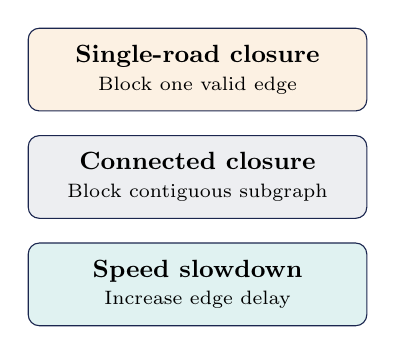
\begin{tikzpicture}[
					>=Stealth,
					ev/.style={
						draw=rPrimary,
						rounded corners=4pt,
						minimum width=4.3cm,
						minimum height=1.05cm,
						align=center,
						font=\small
					}
					]
					\node[ev,fill=rAccent!13](e1){\textbf{Single-road closure}\\[-1pt]\scriptsize Block one valid edge};
					\node[ev,fill=rPrimary!8,below=0.3cm of e1](e2){\textbf{Connected closure}\\[-1pt]\scriptsize Block contiguous subgraph};
					\node[ev,fill=rTeal!12,below=0.3cm of e2](e3){\textbf{Speed slowdown}\\[-1pt]\scriptsize Increase edge delay};
					
				\end{tikzpicture}
			\end{column}
		\end{columns}
		\vspace{0.25cm}
		\takeaway{Language models make the benchmark adversarial; symbolic validation keeps the experiment controlled.}
	\end{frame}
	
	%% 24 -------------------------------------------------------------------------
	\begin{frame}{Plan-hidden events test route adaptation without route leakage}
		\centering
		
\begin{tikzpicture}[
			>=Stealth,
			node distance=8mm,
			b/.style={
				draw=rPrimary,
				fill=rPrimary!8,
				line width=1pt,
				rounded corners=3pt,
				minimum height=1.05cm,
				text width=2.35cm,
				align=center,
				font=\small
			},
			d/.style={
				draw=rTeal,
				fill=rTeal!12,
				line width=1pt,
				rounded corners=3pt,
				minimum height=1.05cm,
				text width=2.85cm,
				align=center,
				font=\small
			}
			]
			\node[b](p0){\textbf{ENHSP}\\Baseline $P_0$};
			\node[d,right=of p0](llm){\textbf{LLM}\\Topology only};
			\node[d,right=of llm](val){\textbf{Python}\\Filter \& Protect $s,g$};
			\node[b,right=of val](p1){\textbf{ENHSP}\\Alternative $P_1$};
			\draw[->,rAccent,line width=1.3pt](p0)--(llm);
			\draw[->,rAccent,line width=1.3pt](llm)--(val);
			\draw[->,rAccent,line width=1.3pt](val)--(p1);
		\end{tikzpicture}
		
		\vspace{0.65cm}
		\begin{columns}[T,onlytextwidth]
			\begin{column}{0.48\textwidth}
				\begin{block}{Baseline Route}
					\[
					P_0=\operatorname{Plan}(G,s,g)
					\]
					\centering\scriptsize\textcolor{rMuted}{Computed offline $\cdot$ Hidden from LLM}
				\end{block}
			\end{column}
			\begin{column}{0.48\textwidth}
				\begin{exampleblock}{Perturbed Route}
					\[
					P_1=\operatorname{Plan}(G_E,s,g)
					\]
					\centering\scriptsize\textcolor{rMuted}{Evaluates route delta: $\Delta(P_0, P_1)$}
				\end{exampleblock}
			\end{column}
		\end{columns}
		\vspace{0.55cm}
		\takeaway{Zero plan leakage guarantees that event relevance is non-trivial.}
	\end{frame}
	
	%% 25 -------------------------------------------------------------------------
	\begin{frame}{Plan-hidden events hit the baseline route in 73.3\% of runs}
		\begin{columns}[T,onlytextwidth]
			\begin{column}{0.51\textwidth}
				\centering
				\includegraphics[height=0.59\textheight,width=0.98\linewidth,keepaspectratio]{figures/500_nodes_event_map.png}
				
				{\scriptsize\color{rMuted}A route before and after a validated LLM-generated disruption.}
			\end{column}
			\begin{column}{0.46\textwidth}
				\textbf{15 valid experiments}\par
				{\scriptsize Graph sizes: 100, 150, and 200 nodes.}
				
				\vspace{0.10cm}
				\metric{rSecondary!10}{73.3\%}{11/15 event sets hit hidden \(P_0\)}\par
				\vspace{0.18cm}
				\metric{rSecondary!14}{6 safeguards}{unsafe closures converted before replanning}\par
				\vspace{0.18cm}
				\metric{rSecondary!10}{60.0\%}{3/5 safe relevant sets changed route}
				
			\end{column}
		\end{columns}
		\vspace{0.08cm}
		\takeaway{Events often hit relevant roads; 15 runs allow only a preliminary conclusion.}
		\note{Time: 60 seconds. Point to the route comparison, then report three numbers. Eleven of fifteen event sets hit at least one baseline road. Among the five relevant cases requiring no safeguard, three changed the road sequence. Six structurally unsafe closures were converted to slowdowns. Emphasise that fifteen experiments are preliminary.}
	\end{frame}
	
	%% 26 -------------------------------------------------------------------------
	\sectionframe{}{Conclusions}{What do the three research questions establish, and where are the remaining limits?}
	\note{Time: 10 seconds. Close the experimental chapters and introduce the final synthesis: direct answers to the three research questions, the main limitations, and the next development step.}
	
	%% 27 -------------------------------------------------------------------------
	\begin{frame}{The results answer all three questions---with clear limits}
		\begin{columns}[T,onlytextwidth]
			\begin{column}{0.55\textwidth}
				\begin{block}{What the experiments establish}
					\begin{itemize}
						\item \textbf{RQ1:} compiled singleton actions reach 2,000 requested nodes.
						\item \textbf{RQ2:} process-preserving controllers extend solved cases to 700 nodes.
						\item \textbf{RQ3:} validated plan-hidden events frequently target relevant roads.
					\end{itemize}
				\end{block}
			\end{column}
			\begin{column}{0.40\textwidth}
				\begin{alertblock}{Current limits}
					\begin{itemize}
						\item one main city topology;
						\item separate controllers and offline events;
						\item 15 final LLM experiments.
					\end{itemize}
				\end{alertblock}
			\end{column}
		\end{columns}
		\vspace{0.95cm}
		\takeaway{ENHSP scales with the modelling detail and parameterisation it must handle.}
		\note{Time: 60 seconds. Answer the research questions directly. Model-side compilation enables the largest tested graphs. Controller-side decomposition preserves richer process semantics. The LLM is useful as a validated event generator. Then acknowledge the three central limitations: one city, separate controllers with offline events, and a small LLM sample.}
	\end{frame}
	
	%% 28 -------------------------------------------------------------------------
	\begin{frame}{A joint controller is the next step}
		\vspace{0.50cm}
		\textbf{One hierarchy prevents fuel and congestion policies from competing.}\par
		\vspace{0.45cm}
		\centering
		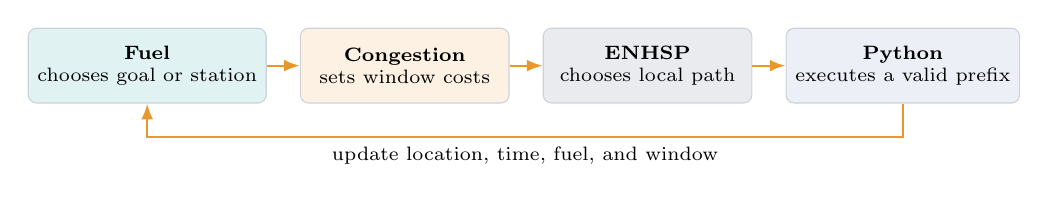
\begin{tikzpicture}[
			node distance=0.42cm,
			box/.style={
				draw=rLine,
				rounded corners=3pt,
				minimum height=0.95cm,
				minimum width=2.65cm,
				align=center,
				font=\scriptsize
			},
			arr/.style={-{Latex[length=2mm]},thick,draw=rAccent}
			]
			\node[box,fill=rTeal!12](fuel){\textbf{Fuel}\\chooses goal or station};
			\node[box,right=of fuel,fill=rAccent!13](cong){\textbf{Congestion}\\sets window costs};
			\node[box,right=of cong,fill=rPrimary!9](plan){\textbf{ENHSP}\\chooses local path};
			\node[box,right=of plan,fill=rSecondary!9](python){\textbf{Python}\\executes a valid prefix};
			\draw[arr](fuel)--(cong);
			\draw[arr](cong)--(plan);
			\draw[arr](plan)--(python);
			\draw[arr](python.south)--++(0,-0.42)-|
			node[pos=0.25,below,font=\scriptsize]{update location, time, fuel, and window}
			(fuel.south);
		\end{tikzpicture}
		
		\vspace{0.95cm}
		\begin{columns}[T,onlytextwidth]
			\begin{column}{0.32\textwidth}
				\metric{rSecondary!10}{Online events}{inject disruptions during route execution}
			\end{column}
			\begin{column}{0.32\textwidth}
				\metric{rPrimary!10}{More cities}{test grid, radial, and irregular topologies}
			\end{column}
			\begin{column}{0.32\textwidth}
				\metric{rAccent!14}{Stronger baselines}{expand LLM tests and routing comparisons}
			\end{column}
		\end{columns}
		
		\vspace{0.25cm}
		\note{Fuel chooses the target. Congestion chooses the costs. ENHSP chooses the path. Python updates the state.}
		\note{Time: 55 seconds. Describe the hierarchy. Fuel decides whether the next target is the final goal or a reachable station. Congestion supplies the costs for the current time window. ENHSP finds the local route and Python executes a node-consistent prefix before updating all state variables. Add online events, more city structures, and stronger baselines.}
	\end{frame}
	
	%% 29 -------------------------------------------------------------------------
	\begin{frame}[plain]
		\begin{tikzpicture}[remember picture,overlay]
			\fill[rPrimary](current page.south west) rectangle (current page.north east);
			\fill[rAccent]([yshift=8mm]current page.west) rectangle ([yshift=11mm]current page.east);
			
			\node[anchor=west,text=white,font=\Huge\bfseries]
			at ([xshift=16mm,yshift=18mm]current page.west){Thank you!};
			\node[anchor=west,text=rAccent,font=\Large]
			at ([xshift=16mm,yshift=-3mm]current page.west){Questions?};
			
			\node[anchor=center,text=white,font=\large\bfseries]
			at ([xshift=-29mm,yshift=31mm]current page.east)
			{GitHub repository};
			\node[fill=white,rounded corners=3pt,inner sep=5pt]
			at ([xshift=-29mm,yshift=9.5mm]current page.east)
			{\qrcode[height=30mm]{https://github.com/GiuseppeRudi/routly-planner}};
		\end{tikzpicture}
		\note{Time: 15 seconds. Thank the audience, invite questions, and point to the QR code for the GitHub repository.}
	\end{frame}
	
\end{document}
